\documentclass[10pt]{beamer}
\usetheme[progressbar=frametitle]{metropolis}

\usepackage [autostyle, english = american]{csquotes}
\DeclareFontShape{OT1}{cmss}{b}{n}{<->ssub * cmss/bx/n}{} 
\usepackage{amsmath}
\usepackage{amssymb}
\usepackage{bm} 

\MakeOuterQuote{"}
\newcommand{\imp}[1]{\textbf{\color{cyan}#1}}

%---------------------------------------------------
% Title 

\title{Estimation of flow trajectories in a multiple lines network}
\subtitle{Experiments with \textit{transports publics de la région lausannoise} (tl) data}
\date{}
\author{Guillaume Guex \\ Romain Loup \\ François Bavaud}
\institute{University of Lausanne}

\begin{document}
	
	%------------------------------------------------------------------
	
	\maketitle
	
	%------------------------------------------------------------------
	
	\begin{frame}{Table of contents}
		\setbeamertemplate{section in toc}[sections numbered]
		\tableofcontents%[hideallsubsections]
	\end{frame}

	%------------------------------------------------------------------
	
	\section[Introduction]{Introduction}
	
	%------------------------------------------------------------------
	
	\begin{frame}{Context}
		
		The \imp{tl dataset}, exploited by Romain Loup for his PhD:
		
		\begin{itemize}
			\item 1 year of data (2019).
			\item 115 millions of passengers.
			\item 42 bus and subway lines.
			\item 1361 stops and 497 "superstops".
			\item Every journey data: traveling time, waiting time, embarking and disembarking passengers at each stops, etc.
		\end{itemize}
		
	\end{frame}

	%------------------------------------------------------------------
	
	\begin{frame}[fragile]{Context}
	\scriptsize
\begin{center}
\begin{verbatim}
     ##   stop_id  stop_name line_id direction order embarkment disembarkment
     ## 1 MALAD_N  Maladière       1         A     1     164558             0
     ## 2 MTOIE_E    Montoie       1         A     2     136236         12705
     ## 3 BATEL_E  Batelière       1         A     3     203045         13409
     ## 4 RTCOU_E Riant-Cour       1         A     4     156015         24909
      
     ##    stop_id  stop_name line_id direction order embarkment disembarkment
     ## 42 RTCOU_O Riant-Cour       1         R    19      23634        132201
     ## 43 BATEL_O  Batelière       1         R    20      13707        168884
     ## 44 MTOIE_O    Montoie       1         R    21       4259        128255
     ## 45 MALAD_N  Maladière       1         R    22          0        146798
\end{verbatim}

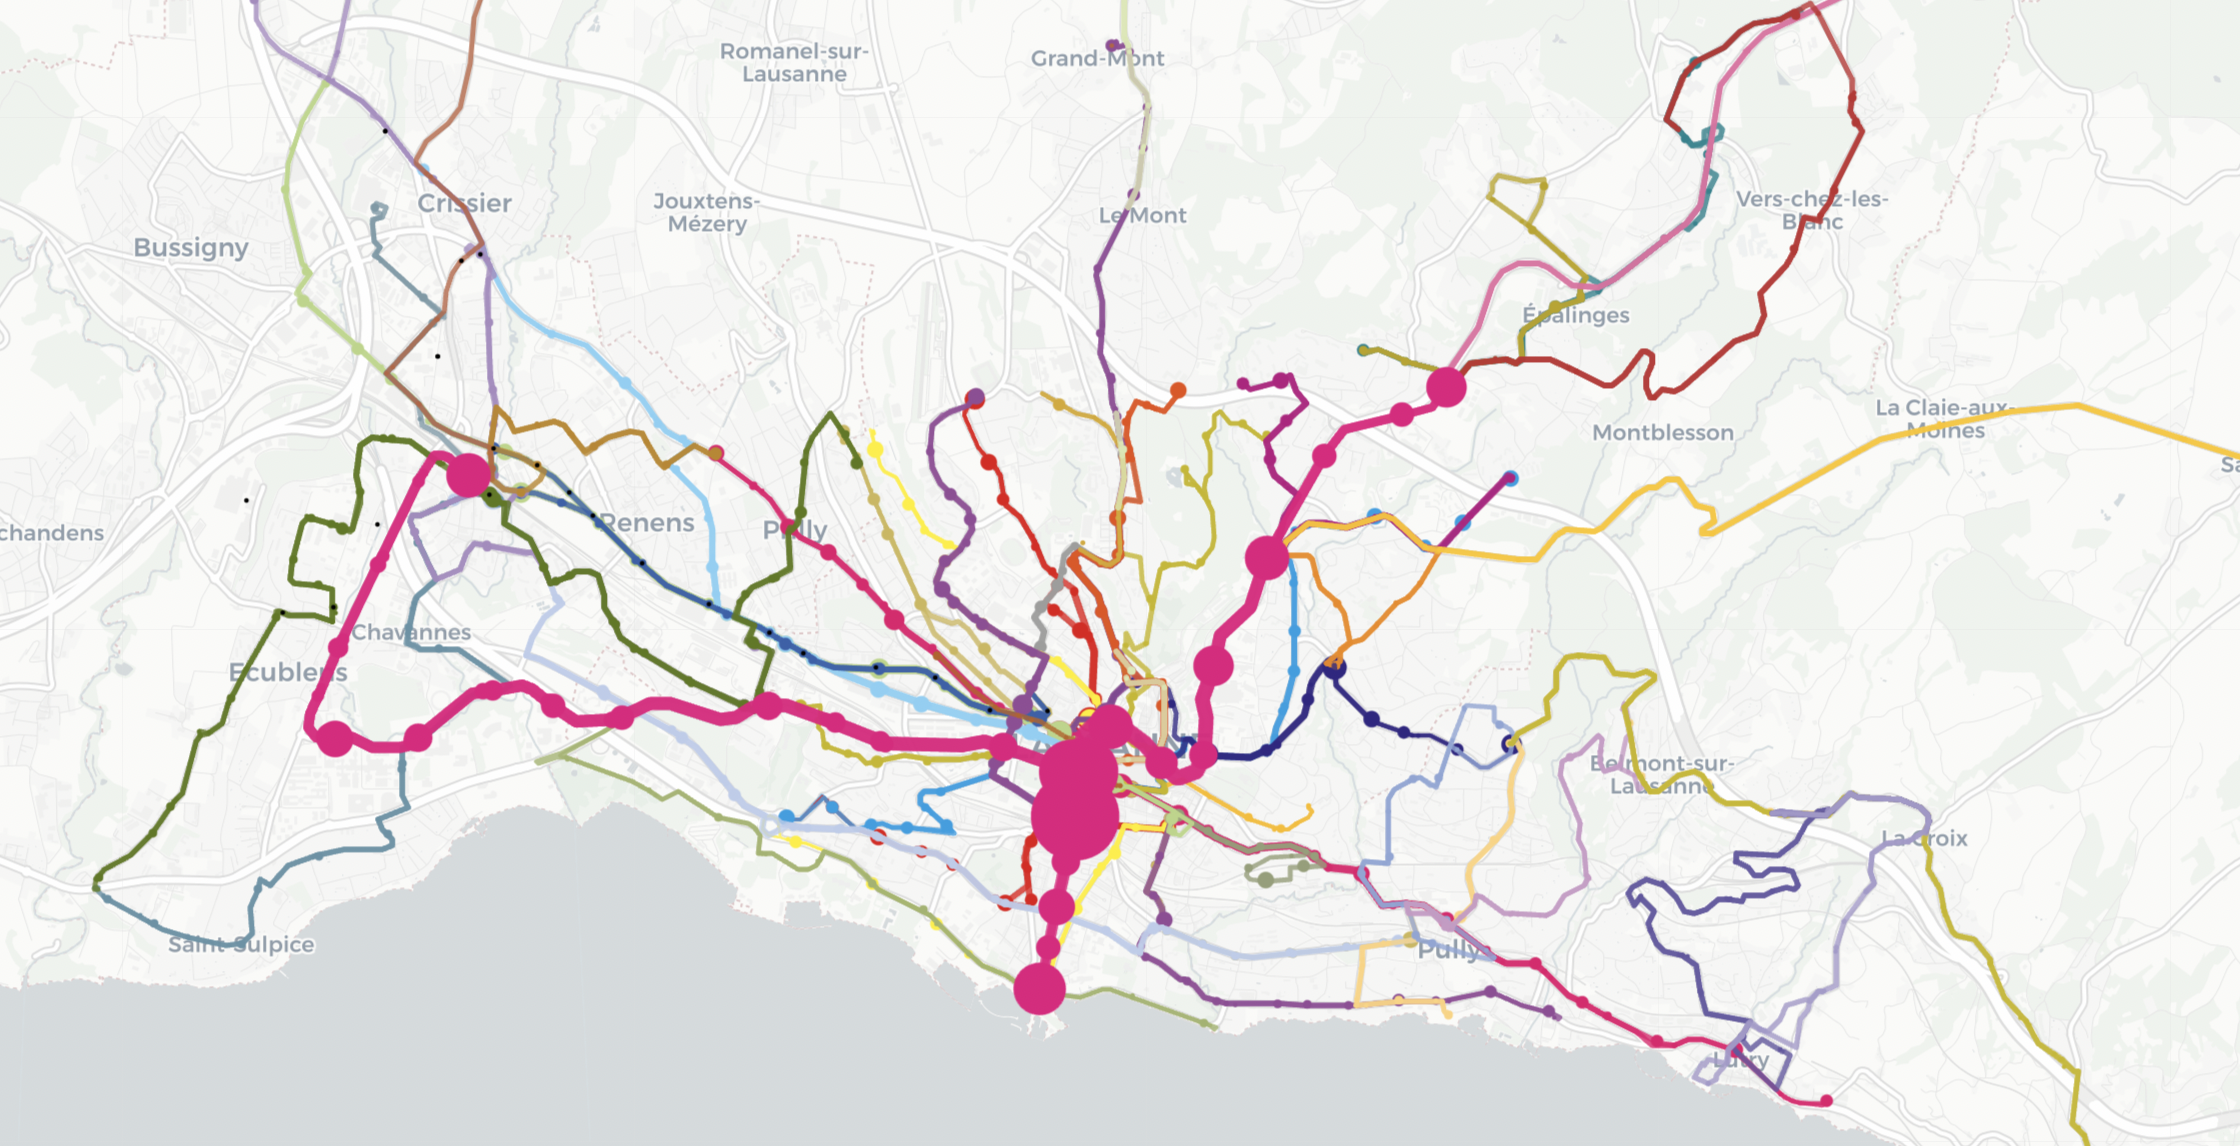
\includegraphics[width=0.7\textwidth]{img/tl_network.png}
\end{center}
	\end{frame}
	
	%------------------------------------------------------------------
	
	\begin{frame}{The multiple lines network}
		\begin{columns}
			\begin{column}{0.5\textwidth}
				Having only lines data, the structure is a \imp{disconnected oriented graph}. \linebreak
				
				In addition to \imp{line edges}, it is possible to construct \imp{transfer edges} to make the graph connected, by using, e.g.,
				\begin{itemize}
					\item Superstops names,
					\item Pedestrian time,
					\item Euclidean distance.
				\end{itemize} 
				\vspace{0.4cm}
				With transfer edges, we have a \imp{unilaterally connected graph}.
			\end{column}
			\begin{column}{0.5\textwidth} 
				\begin{center}
					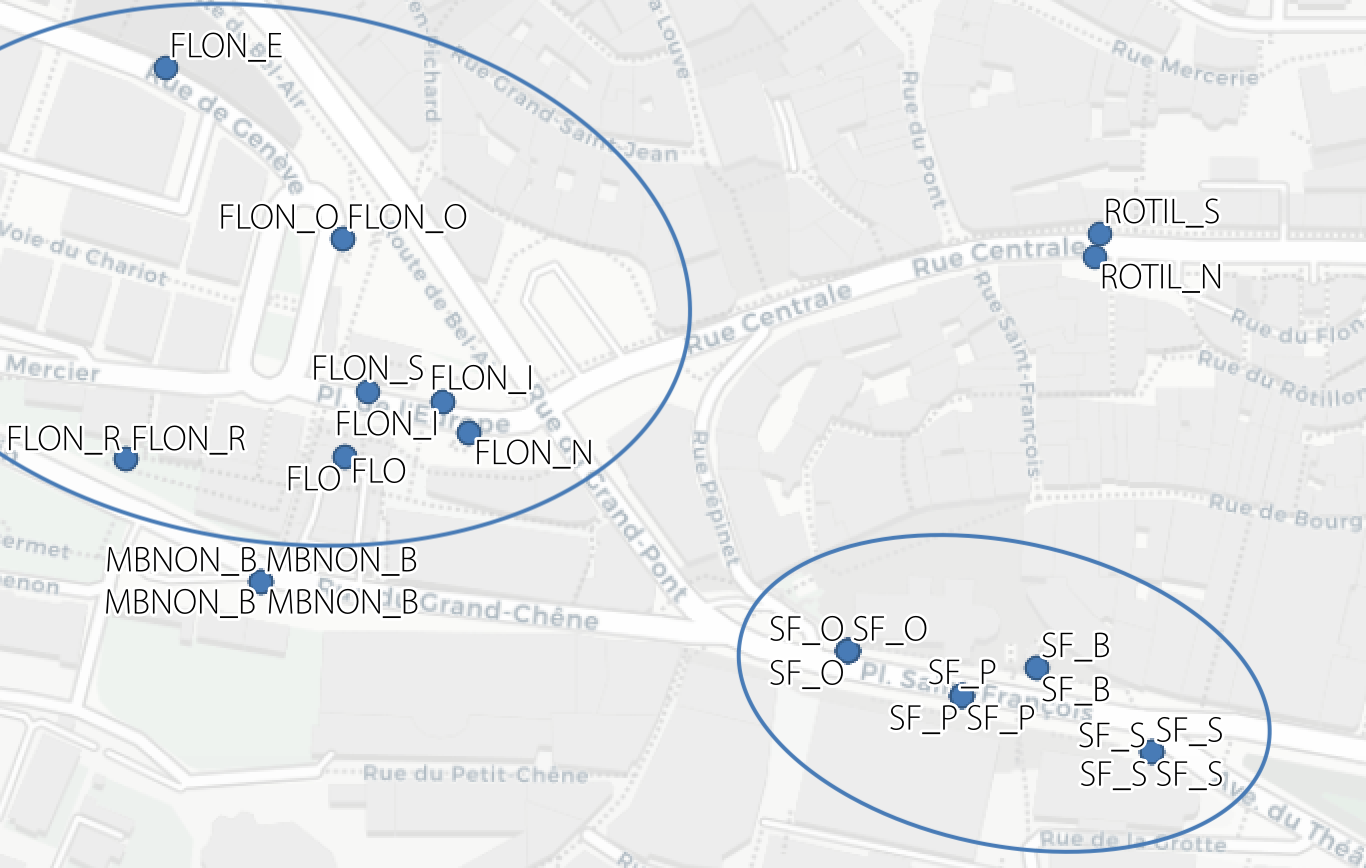
\includegraphics[width=0.8\textwidth]{img/stop_area_c.png} \\
					\vspace{0.5cm}
					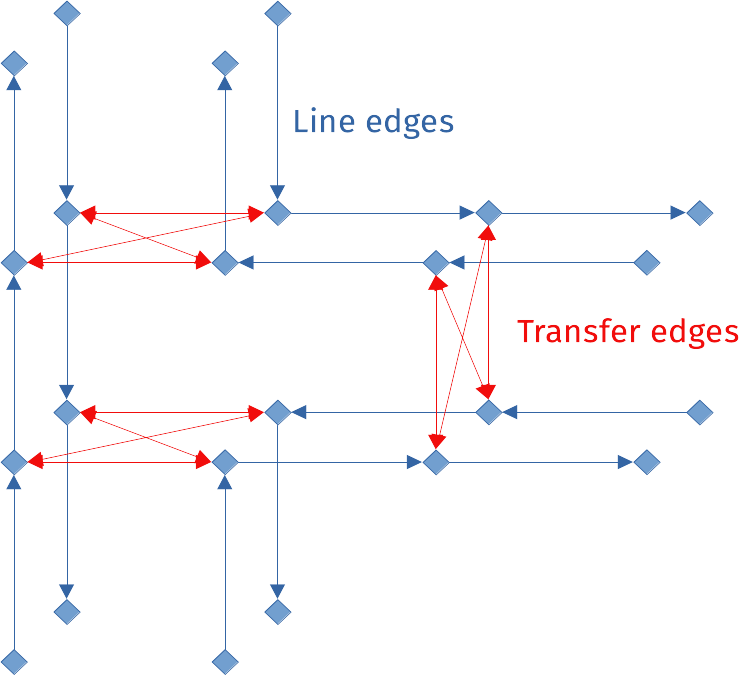
\includegraphics[width=0.7\textwidth]{img/edge_type2.png}
				\end{center}
			\end{column}
		\end{columns}
	\end{frame}
	
	%------------------------------------------------------------------

	\begin{frame}{Problematic}
		
		This dataset offers multiple axes of research. In this presentation, we focus on one question: \\
		\vspace{0.6cm}
		\begin{quotation}
			\large
			Knowing \imp{(1) the network structure} and \imp{(2) the number of passengers embarking and disembarking at each stop}, can we deduce \imp{trajectories of the passengers} in the network ?
		\end{quotation}
		\normalsize
		\vspace{0.4cm}
		Short answer: {\large \imp{No}}.
	\end{frame}

	%------------------------------------------------------------------
	
	\begin{frame}

		\begin{center}
			\huge Thank you for your attention ! \\
			Questions ? \\
			\vspace{1cm}
			\small
			(just kidding)
		\end{center}
		
		
	\end{frame}
	
	%------------------------------------------------------------------
	
	\begin{frame}{Problematic}
		
		Exact trajectories are impossible to know, but, with additional assumptions, we can produce  \imp{estimations} of them. \\
		\vspace{0.4cm}
		We divide this problematic into two parts:
		\begin{itemize}
			\item Estimation of trajectories on a \imp{single line}.
			\item Estimation of trajectories on the \imp{multiple lines network}.
		\end{itemize}
		
	\end{frame}
	
	%------------------------------------------------------------------
	
	\section{The single line problem}
	
	%------------------------------------------------------------------
	
	\begin{frame}{Formal problem definition}
		Let a line (in one direction), which have $n$ stops, indexed regarding line order. Let \imp{$\bm{\rho}_\text{in} = (\rho^\text{in}_s)$} and \imp{$\bm{\rho}_\text{out} = (\rho^\text{out}_t)$} be two vectors representing, respectively, the \imp{passengers entering and leaving the line at each stop}. \\
		\vspace{0.4cm}
		We search a $(n \times n)$ \imp{origin-destination matrix $\mathbf{N} = (n_{st})$} where components represents
		$$
			{\color{cyan} n_{st} = \text{"the number of passengers entering line at $s$ and leaving at $t$"}}.
		$$
		These components must verify
		\begin{enumerate}
			\item $n_{st} \geq 0$,
			\item $n_{s\bullet} = \rho^\text{in}_s$,
			\item $n_{\bullet t} = \rho^\text{out}_t$.
		\end{enumerate}
		\small ($\bullet$ indicates a sum on the replaced index)
	\end{frame}
	
	%------------------------------------------------------------------
	
	\begin{frame}{Formal problem definition}
		\small
		It reads
		$$
		\mathbf{N} = \bordermatrix{
			& \rho^\text{out}_1 & \rho^\text{out}_2  & \cdots & \rho^\text{out}_{n-1} & \rho^\text{out}_n   \cr
			\rho^\text{in}_1 & n_{11} & n_{12} & \cdots & n_{1,n-1} & n_{1n} \cr
			\rho^\text{in}_2 & n_{21} & n_{22} & \cdots & n_{2,n-1} & n_{2n} \cr
			\vdots & \vdots & \vdots & \ddots & \vdots & \vdots \cr
			\rho^\text{in}_{n-1} & n_{n-1,1} & n_{n-1,2} & \cdots & n_{n-1,n-1} & n_{n-1,n} \cr
			\rho^\text{in}_{n} & n_{n,1} & n_{n,2} & \cdots & n_{n,n-1} & n_{n,n}}
		$$
		
		In fact, we already know that some components are null
		$$
		\mathbf{N} = \bordermatrix{
			& \imp{0} & \rho^\text{out}_2  & \cdots & \rho^\text{out}_{n-1} & \rho^\text{out}_n \cr
			\rho^\text{in}_1 & \imp{0} & n_{12} & \cdots & n_{1,n-1} & n_{1n} \cr
			\rho^\text{in}_2 & \imp{0} & \imp{0} & \ddots & \cdot & n_{2n} \cr
			\vdots & \vdots & \vdots & \ddots & \ddots & \vdots \cr
			\rho^\text{in}_{n-1} & \imp{0} & \imp{0} & \cdots & \imp{0} & n_{n-1,n} \cr
			\imp{0} & \imp{0} & \imp{0} & \cdots & \imp{0} & \imp{0}}
		$$
	\end{frame}
	
	%------------------------------------------------------------------
	
	\begin{frame}{Formal problem definition}
		
		In this form, the problem is \imp{ill posed}, because it has multiple acceptable solutions. An exemple of solution is to make passengers follow a \imp{first in, first out (FIFO)} scheme. \\
		\vspace{0.4cm}
		A principle of mathematical modeling is to find the solution which makes the \imp{least assumptions about passenger behavior}, in other words the \imp{maximum entropy solution}. \\
		\vspace{0.4cm}
		In this case, it translates by supposing that there is the \imp{same probability of leaving the line for every passenger which have traveled at least one stop}.
		
	\end{frame}
	
	%------------------------------------------------------------------
	
	\begin{frame}{Solution with Markov chain modeling}
		
		We can then model passenger flow with a \imp{Markov chain}:
		
		\begin{center}
			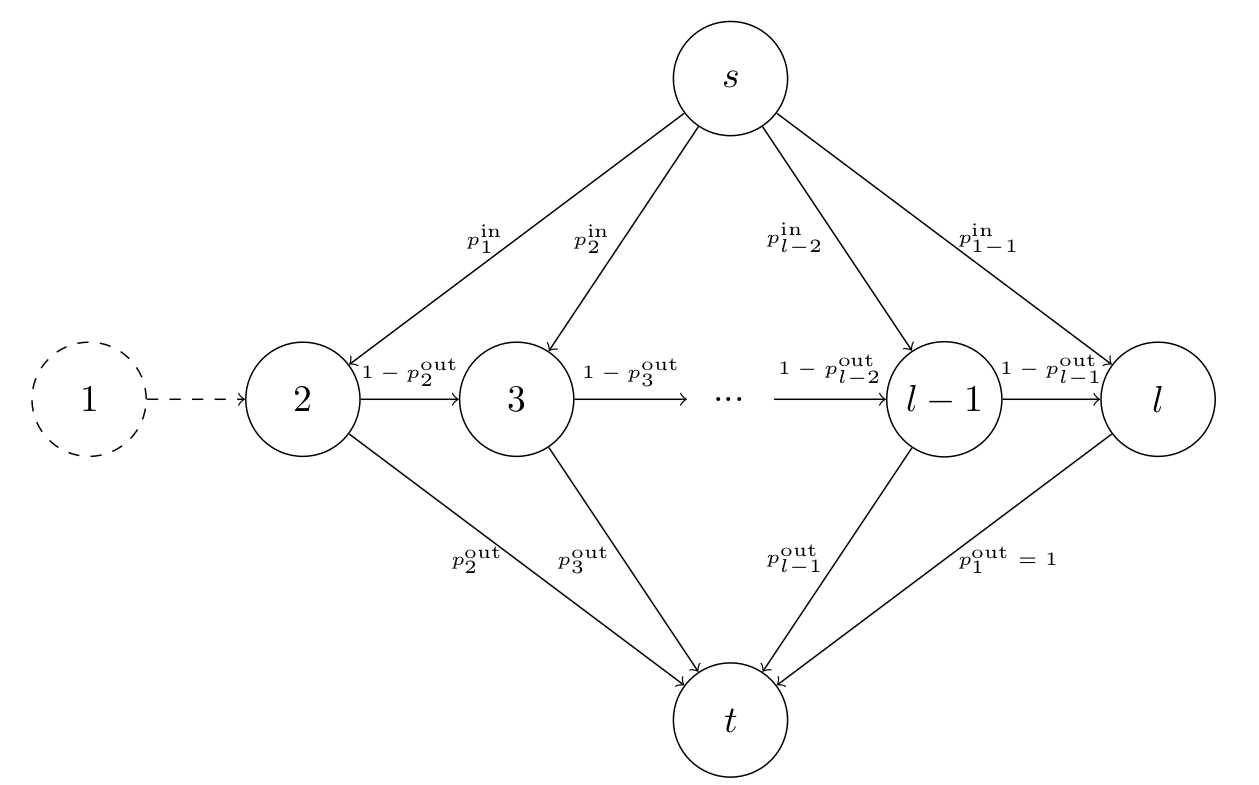
\includegraphics[width=0.8\linewidth]{img/line_markov.png} 
		\end{center}
		
		with $p^\text{in}_i = \frac{\rho^\text{in}_i}{\rho^\text{in}_\bullet}$ and $p^\text{out}_i = \frac{\rho^\text{out}_i}{\sum_{1 \leq k \leq (i-1)} (\rho^\text{in}_k - \rho^\text{out}_k)}$.
	\end{frame}
	
	%------------------------------------------------------------------
	
	\begin{frame}{Solution with Markov chain modeling}

		\begin{center}
			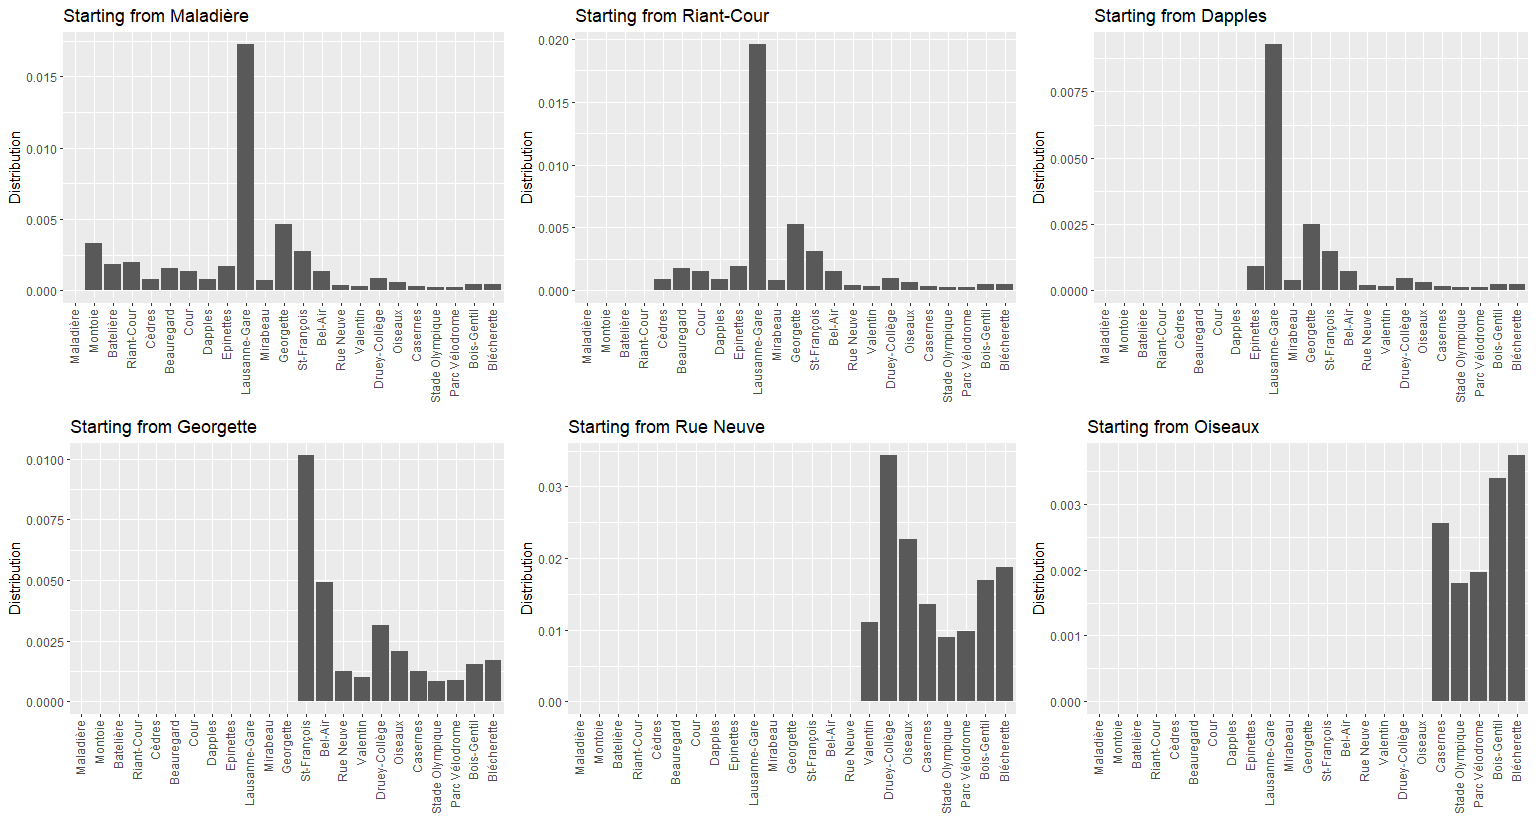
\includegraphics[width=\textwidth]{img/stop_distributions.png} 
		\end{center}
	
	\end{frame}
	
	%------------------------------------------------------------------
	
	\begin{frame}{Solution with Markov chain modeling}
		
		\begin{center}
			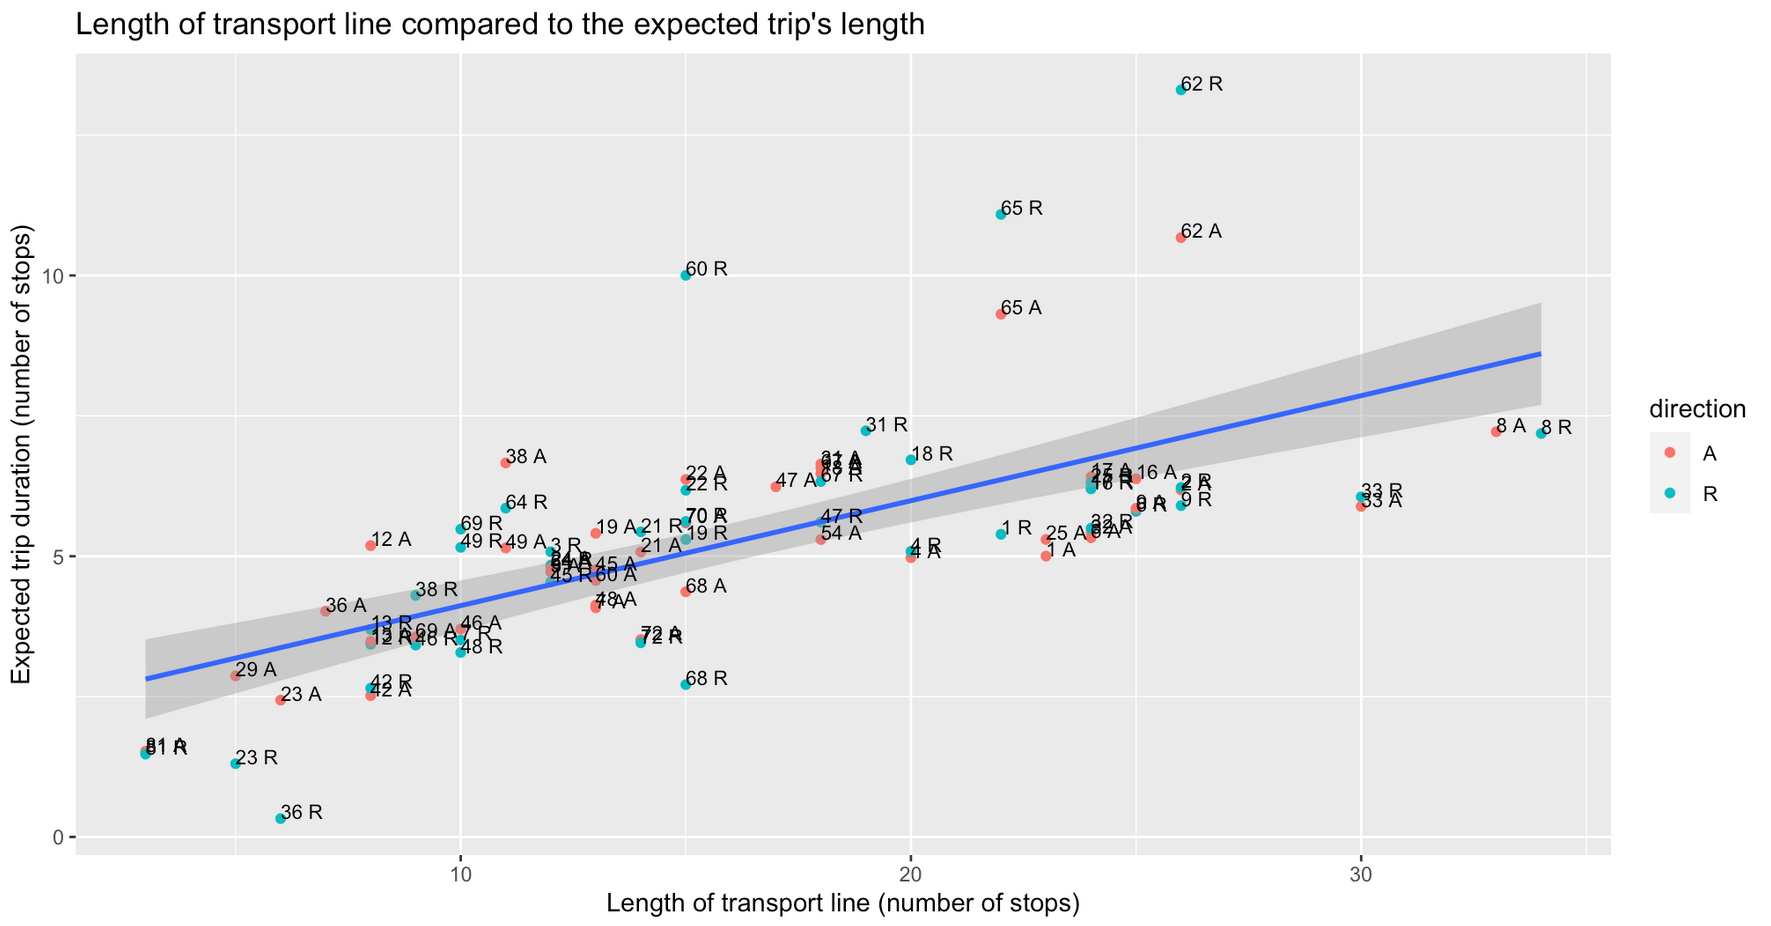
\includegraphics[width=\textwidth]{img/length_exp.png} 
		\end{center}
		
	\end{frame}
	
	%------------------------------------------------------------------
	
	\section{Iterative proportial fitting}
	
	%------------------------------------------------------------------
	
	\begin{frame}{Iterative proportional fitting}
	
	The same solution can be obtained with the \imp{iterative proportional fitting (IPF)} algorithm [Bishop et al., 1975]. Let 
	\begin{enumerate}
		\item $\mathbf{P} = (p_{ij})$ a $(n \times m)$ matrix, 
		\item $\mathbf{u} = (u_i)$ a n-length vector, and 
		\item $\mathbf{v} = (v_i)$ a m-length vector,
	\end{enumerate}
	all of them with strictly positive components. We can find two vectors $\mathbf{a} = (a_i)$ and $\mathbf{b} = (b_i)$ such that the matrix $\mathbf{Q} = (q_{ij})$, defined with
	$$
		q_{ij} = a_i b_j p_{ij},
	$$
	verifies
	\begin{itemize}
		\item $q_{i\bullet} = u_i$,
		\item $q_{\bullet j} = v_j$,
		\item $K(\mathbf{Q}| \mathbf{P}) := \sum_{ij} \frac{q_{ij}}{q_{\bullet \bullet}} \log \left( \frac{q_{ij} / q_{\bullet \bullet}}{p_{ij} / p_{\bullet \bullet}} \right)$ is minimum.
	\end{itemize}
	\end{frame}
	
	%------------------------------------------------------------------
	
	\begin{frame}{Solution with iterative proportional fitting}
		
		In our context, it means that if we define an \imp{origin-destination affinity matrix $\mathbf{S} = (s_{st})$} with 
			$$
				\mathbf{S} = \left( \begin{array}{ccccc}
				0 & 1 & 1 & \cdots & 1 \\
				0 & 0 & 1 & \cdots & 1 \\
				\vdots & \vdots & \ddots & \ddots & \vdots \\
				0 & 0 & \cdots & 0 & 1 \\
				0 & 0 & \cdots & 0 & 0 
				\end{array} \right)
			$$
		we can find the \imp{same maximum entropy solution with iterative proportional fitting}, i.e., we can find $\mathbf{a} = (a_s)$ and $\mathbf{b} = (b_t)$, such that $n_{ij} = a_s b_t s_{st}$ verifies
		\begin{enumerate}
			\item $n_{s\bullet} = \rho^\text{in}_s$,
			\item $n_{\bullet t} = \rho^\text{out}_t$,
			\item $K(\mathbf{N}| \mathbf{S})$ is minimum.
		\end{enumerate}
		\small (a small number $\epsilon$ has to be added on null components).
	\end{frame}
	
	%------------------------------------------------------------------
	
	\begin{frame}{Solution with iterative proportional fitting}
		By \imp{decreasing (resp. increasing) $s_{st}$}, we \imp{reduce (resp. expand)} the resulting number of passengers going from $s$ to $t$ obtained with IPF. \\
		\vspace{0.4cm}
		Thus, this approach is more \imp{flexible}, because we could give a \imp{specific affinity matrix $\mathbf{S} = (s_{st})$}, based on other data (additional assumptions).\\
		\vspace{0.4cm}
		The relationship $n_{st} = a_s b_t s_{st}$ can be seen as a \imp{gravity model} (still to investigate).
	\end{frame}
		
	%------------------------------------------------------------------
	
	\section{The multiple lines problem}
	
	%------------------------------------------------------------------
	
	\begin{frame}{The multiple lines problem}
		
		In this problem, the whole multiple lines network is used. Let us recall that it is composed of \imp{line edges} and \imp{transfer edges}.
		
		\begin{center}
			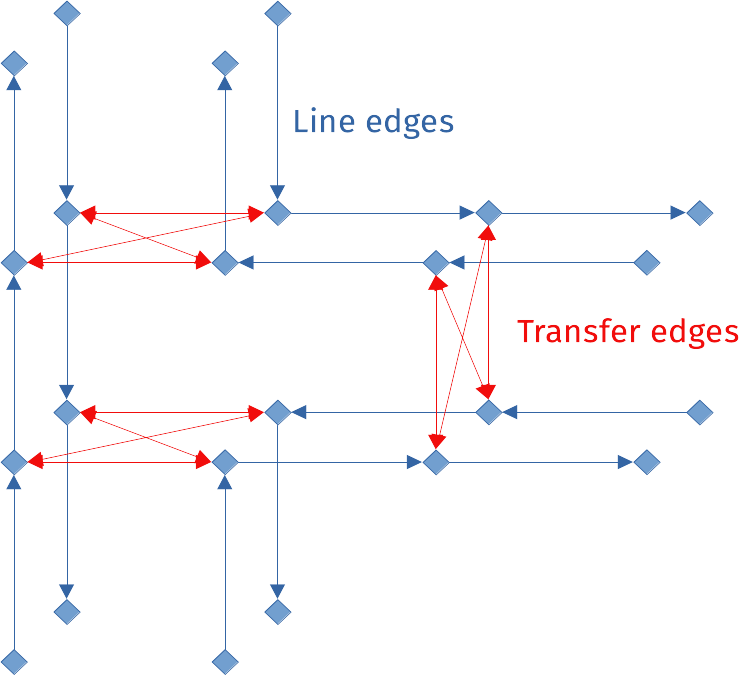
\includegraphics[width=0.45\textwidth]{img/edge_type2.png}
		\end{center}
	
		It is not possible to use a Markov chain modeling in this case, but the \imp{iterative proportional fitting} approach is still valid. However, there are \imp{additional difficulties}.
		
	\end{frame}
	
	%-----------------------------------------------^-------------------
	
	
	\begin{frame}{Flow behavior}
		
		The first difficulty is that there are generally \imp{multiple routes} to go from node $s$ to $t$. This can be solved by making a new assumption. \\
		\vspace{0.4cm}
		In the multiple lines network, we suppose that passengers take \imp{shortest-paths} in order to reach node $t$ from node $s$. \\
		\vspace{0.4cm}
		If multiple shortest-paths exists between $s$ and $t$, the passenger flow is \imp{divided equally} among them.
		
	\end{frame}
	
	%------------------------------------------------------------------
	
	\begin{frame}{Flow behavior}
		
		This assumption unlocks a very useful property. If we have an \imp{origin-destination matrix} $\mathbf{N} = (n_{st})$, we can compute the $(n \times n)$ \imp{flow matrix on edges $\mathbf{X} = (x_{ij})$}. \\
		\vspace{0.6cm}
		\begin{columns}
			\small
			\begin{column}{0.7\textwidth}
				$$
				\hspace{1cm} \mathbf{N} = \left( \begin{array}{ccccc}
				0 & 13055 & 243 & \cdots & 144 \\
				3498 & 0 & 24429 & \cdots & 7523 \\
				\vdots & \vdots & \ddots & \ddots & \vdots \\
				1508 &  & \cdots & 0 & 5093 \\
				8903 & 6343 & \cdots & 53 & 0 
				\end{array} \right) \rightarrow 
				$$ 
			\end{column}
			\begin{column}{0.6\textwidth}
				\hspace{0.5cm} 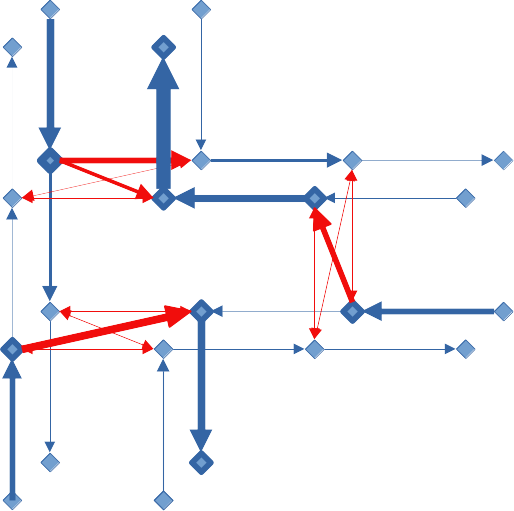
\includegraphics[width=0.5\textwidth]{img/flow_computed.png}
			\end{column}
		\end{columns}
	\end{frame}
	
	%------------------------------------------------------------------
	
	\begin{frame}{The flow in/out lines/network}
		
		A second problem is that we have to distinguish between
		
		\begin{itemize}
			\item The passengers \imp{entering and leaving lines} at each stop, represented by vectors \imp{$\bm{\rho}_\text{in}$} and \imp{$\bm{\rho}_\text{out}$}, which are \imp{measured}, and 
			\item The passengers \imp{entering and leaving the network} at each stop, represented by vectors \imp{$\bm{\sigma}_\text{in}$} and \imp{$\bm{\sigma}_\text{out}$}, which are \imp{unknown}.
		\end{itemize}
	
		At each stop $i$, we have 
		
		\begin{align*}
			\rho^\text{in}_i &= \sigma^\text{in}_i + x^\text{B}_{\bullet i}, \\
			\rho^\text{out}_i &= \sigma^\text{out}_i + x^\text{B}_{i \bullet},
		\end{align*}
		
		where 
		\begin{itemize}
			\item $x^\text{B}_{\bullet i}$ is the \imp{transfer flow entering the node $i$} and
			\item $x^\text{B}_{i \bullet}$ is the \imp{transfer flow leaving the node $i$}.
		\end{itemize}
	\end{frame}
	
	%------------------------------------------------------------------
	
	\begin{frame}{The flow in/out lines/network}
		\begin{center}
			\hspace{0.1cm} 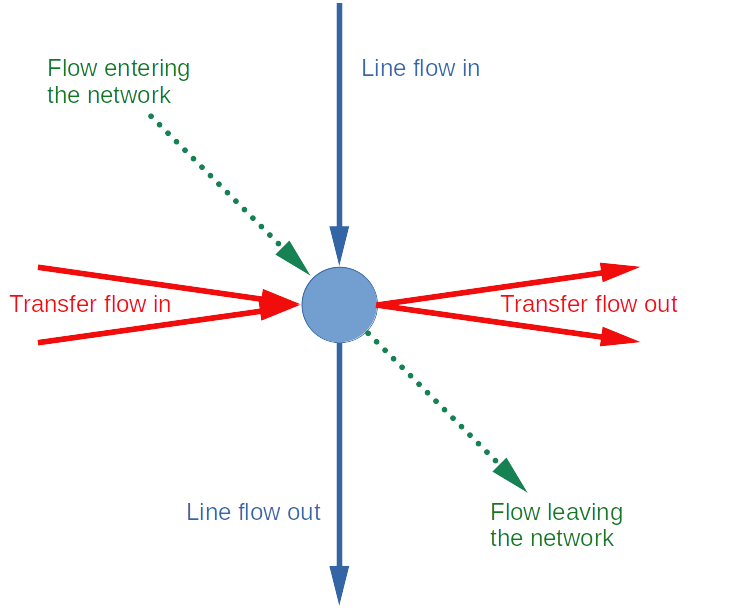
\includegraphics[width=0.8\textwidth]{img/flow_balance.png}
		\end{center}
	\end{frame}
	
	%------------------------------------------------------------------
	
	\begin{frame}{The flow in/out lines/network}
		\begin{center}
			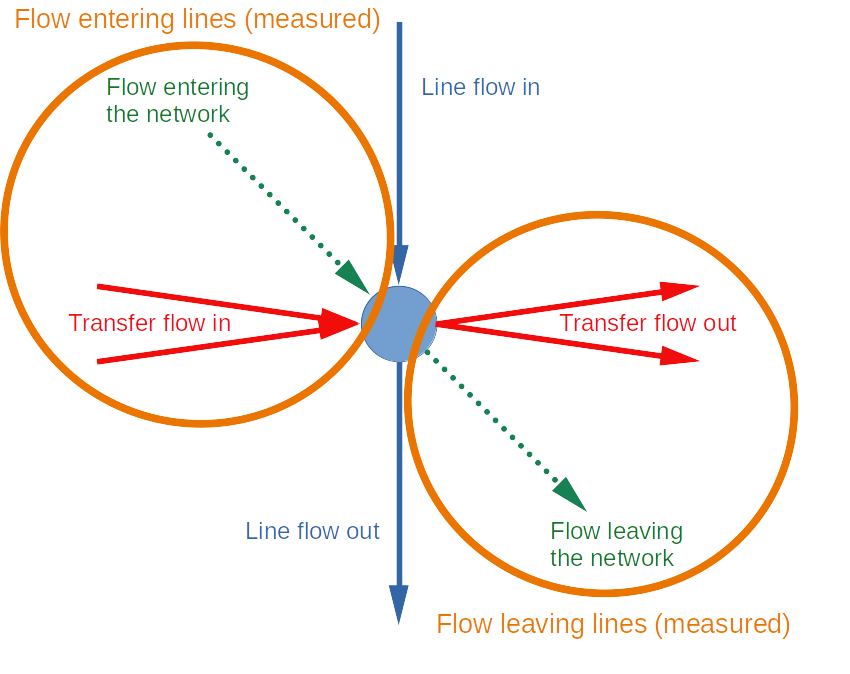
\includegraphics[width=0.9\textwidth]{img/flow_measured.png}
		\end{center}
	\end{frame}
	
	%------------------------------------------------------------------
	
	\begin{frame}{The flow in/out lines/network}
		If we know \imp{transfer flow on edges}, i.e. $\mathbf{X}_\text{B} = (x^\text{B}_{ij})$, we can \imp{compute the flow entering/leaving the network}, $\bm{\sigma}_\text{in}$ and $\bm{\sigma}_\text{in}$. \\
		\vspace{0.4cm}
		The flow entering/leaving the lines, $\rho^\text{in}_i$ and $\rho^\text{out}_i$, acts as \imp{constraints on the in/out transfer flow}, $x^\text{B}_{\bullet i}$ and $x^\text{B}_{i \bullet}$.\\
		\vspace{0.4cm}
		When there are no transfers on $i$, we have $\sigma^\text{in}_i = \rho^\text{in}_i$ and  $\sigma^\text{out}_i = \rho^\text{out}_i$. \\
	\end{frame}
	
	%------------------------------------------------------------------
	
	\begin{frame}{Algorithm outline}
		
		Let us make an outline for the \imp{iterative Algorithm}. There are \imp{4 steps} at each iteration: \\
		\footnotesize
		\begin{align}
			\left. \begin{array}{r} 
				{\color{cyan} \text{OD affinity matrix } \mathbf{S}} \\
				{\color{cyan} \text{Flow in the network } \bm{\sigma}_\text{in}} \\
				{\color{cyan} \text{Flow out the network } \bm{\sigma}_\text{out}}
			\end{array} \right\}  &\overset{IPF}{\longrightarrow} \text{OD matrix } \mathbf{N} \\
			\begin{array}{r}
			\text{OD matrix } \mathbf{N}
			\end{array} &\overset{SP}{\longrightarrow} \text{Transfer flow } \mathbf{X}_\text{B} \\
			\left. \begin{array}{r} 
			\text{Transfer flow } \mathbf{X}^\text{B} \\
			\text{Flow in lines } \bm{\rho}_\text{in} \\
			\text{Flow out lines } \bm{\rho}_\text{out}
			\end{array} \right\}  &\overset{\text{Constraints}}{\longrightarrow} 
			\left\{ \begin{array}{l}
			\text{Allowed transfer flow } \widetilde{\mathbf{X}}_\text{B} \\
			{\color{cyan} \text{Flow in the network } \bm{\sigma}_\text{in}} \\
			{\color{cyan} \text{Flow out the network } \bm{\sigma}_\text{out}}
			\end{array} \right. \\
			\left. \begin{array}{r} 
			\text{Transfer flow } \mathbf{X}_\text{B} \\
			 \text{Allowed transfer flow } \widetilde{\mathbf{X}}_\text{B}
			\end{array} \right\}  &\overset{\text{Affinity update}}{\longrightarrow} {\color{cyan} \text{OD affinity matrix } \mathbf{S}}
		\end{align}	
	\end{frame}
	
	%------------------------------------------------------------------
	
	\begin{frame}{Step 1: iterative proportional fitting}
		
		At the beginning of the algorithm, we have to set 
		\begin{itemize}
			\item An \imp{initial flow in the network }. We can set it to $\bm{\sigma}^\text{init}_\text{in} = \bm{\rho}_\text{in}$,
			\item An \imp{initial flow out the network }. We can set it to $\bm{\sigma}^\text{init}_\text{out} = \bm{\rho}_\text{out}$,
			\item An \imp{initial affinity matrix between origin-destination}, $\mathbf{S}^\text{init}$.
		\end{itemize}  
	
		The initial affinity matrix $\mathbf{S}^\text{init} = (s^\text{init}_{st})$ is crafted in order to have
		\begin{itemize}
			\item $s^\text{init}_{st} = 1$, if going from $s$ to $t$ is a \imp{valid trajectory} for using the network,
			\item $s^\text{init}_{st} = 0$, otherwise.
		\end{itemize}
		
		It now possible to obtain a first origin-destination matrix $\mathbf{N}$ with \imp{iterative proportional fitting}.
		
	\end{frame}
	
	%------------------------------------------------------------------
	
	\begin{frame}{Step 2: shortest-paths flow}
		
		In this step, we use the assumption that passengers use \imp{shortest-paths} in the network to obtain flow on edges, and in particular, \imp{flow on transfer edges}:
		$$
			\mathbf{N} \longrightarrow \mathbf{X}_\text{B}
		$$ 
		\vspace{0.6cm}
		\begin{columns}
			\small
			\begin{column}{0.7\textwidth}
				$$
				\hspace{1cm} \mathbf{N} = \left( \begin{array}{ccccc}
				0 & 13055 & 243 & \cdots & 144 \\
				3498 & 0 & 24429 & \cdots & 7523 \\
				\vdots & \vdots & \ddots & \ddots & \vdots \\
				1508 &  & \cdots & 0 & 5093 \\
				8903 & 6343 & \cdots & 53 & 0 
				\end{array} \right) \rightarrow 
				$$ 
			\end{column}
			\begin{column}{0.6\textwidth}
				\hspace{0.5cm} 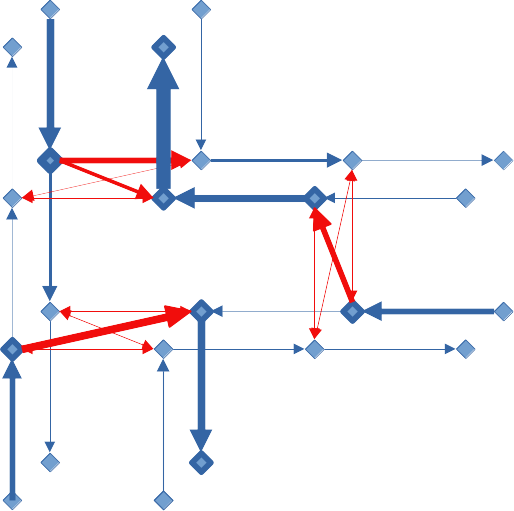
\includegraphics[width=0.5\textwidth]{img/flow_computed.png}
			\end{column}
		\end{columns}
	\end{frame}
	
	%------------------------------------------------------------------
	
	\begin{frame}{Step 3: corrected transfer flow}
		
		This transfer flow $\mathbf{X}_\text{B}$ could be used to update $\bm{\sigma}_\text{in}$ and $\bm{\sigma}_\text{out}$, with 
		\begin{align*}
			\sigma^\text{in}_i &= \rho^\text{in}_i - x^\text{B}_{\bullet i}, \\
			\sigma^\text{out}_i &= \rho^\text{out}_i - x^\text{B}_{i \bullet}.
		\end{align*}
		However, there is \imp{no guarantee that the transfer flow do not exceed limits given by $\bm{\rho}_\text{in}$ and $\bm{\rho}_\text{in}$}.
		\begin{center}
			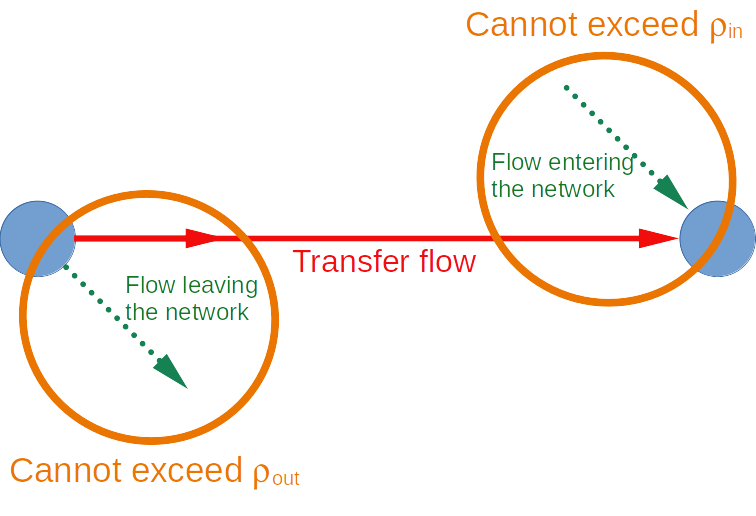
\includegraphics[width=0.7\textwidth]{img/flow_constrained.png}
		\end{center}
	\end{frame}
	
	%------------------------------------------------------------------
	
	\begin{frame}{Step 3: allowed transfer flow}
		
		For each $x^\text{B}_{ij}$, we use $\rho^\text{out}_i$ and $\rho^\text{in}_j$ in order to compute a \imp{allowed transfer flow  $\widetilde{x}_{ij}^\text{B}$}, with  $\widetilde{x}_{ij}^\text{B} \leq x_{ij}^\text{B}$. There are multiple choices:
		
		\begin{enumerate}
			\item \imp{Constraint thresholds} could be reachable.
			\item We can set a \imp{percentage limit} for the transfer flow among the flow in/out of the lines.
			\item We can set a \imp{soft limit} to the transfer flow, with, e.g., an exponential law.
		\end{enumerate}
		
		When this allowed flow is computed, $\bm{\sigma}_\text{in}$ and $\bm{\sigma}_\text{out}$ can be \imp{updated} with 
		\begin{align*}
			\sigma^\text{in}_i &= \rho^\text{in}_i - \widetilde{x}^\text{B}_{\bullet i}, \\	\sigma^\text{out}_i &= \rho^\text{out}_i - \widetilde{x}^\text{B}_{i \bullet}.
		\end{align*}
	\end{frame}
	
	%------------------------------------------------------------------
	
	\begin{frame}{Step 4: Affinity update}
		
		What about the \imp{excess flow on transfer edges}, i.e., $x^\text{B}_{ij} - \widetilde{x}^\text{B}_{ij}$ ? \\
		\vspace{0.4cm}
		Note that we only updated \imp{margins distribution}, but we also need a way to reduce \imp{dependencies} between particular $s$ and $t$. \\
		\vspace{0.4cm}
		Having flow following \imp{shortest-paths}, we know which couples $s, t$ are "responsible" for the excess flow on edge $(i, j)$.
		\begin{center}
			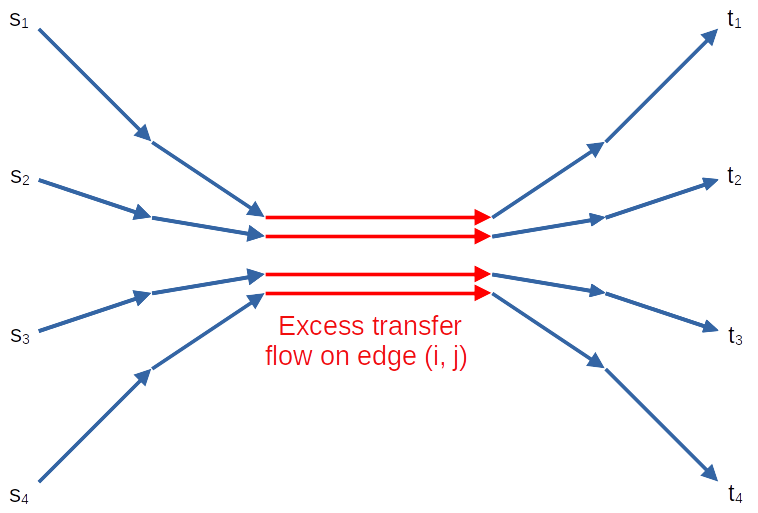
\includegraphics[width=0.6\textwidth]{img/excess_flow.png}
		\end{center}
	\end{frame}
	
	%------------------------------------------------------------------
	
	\begin{frame}{Step 4: Affinity update}
		
		On each transfer edge, we can compute the \imp{proportion of allowed flow}:
		$$
			p^\text{allowed}_{ij} = \frac{\widetilde{x}_{ij}^\text{B}}{x_{ij}^\text{B}}
		$$
		Each transfer edge $(i,j)$ transmits this proportion $p^\text{allowed}_{ij}$ to all couples $s,t$ that use this edge. Each couple $s,t$ receiving a reduced proportion have to \imp{reduce its affinity $s_{st}$}. \\
		\vspace{0.4cm}
		Each couple $s,t$ receives a \imp{list of proportion of allowed flow}, from all transfer edges on its shortest-path. The \imp{update factor for the affinity $s_{st}$} is constructed by using the minimum allowed flow received.
		$$
			s^\text{new}_{st} = \min\{p^\text{allowed}_{i_1, j_1}, \ldots, p^\text{allowed}_{i_k, j_k} \} \cdot s^\text{old}_{st}
		$$
	\end{frame}
	
	%------------------------------------------------------------------
	
	\begin{frame}{Step 4: Affinity update}
		\begin{center}
			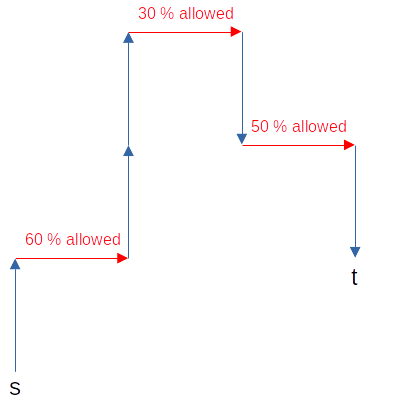
\includegraphics[width=0.7\textwidth]{img/allowed_flow.png} \\
			In this example, $s^\text{new}_{st} = 0.3 \cdot s^\text{old}_{st}$
		\end{center}
	\end{frame}
	
	%------------------------------------------------------------------

	
	\section{Results (demo)} 
	
	%------------------------------------------------------------------
	
	
	\section{Conclusion} 
	
	%------------------------------------------------------------------
	
	\begin{frame}{Conclusion}
		
		As it is still a work in progress, the conclusion takes the form of a to-do list:
		\begin{itemize}
			\item \imp{Optimizing} speed/memory (almost done).
			\item Running the algorithm on \imp{all lines}.
			\item Testing multiple \imp{initial conditions} and \imp{hyperparameter values}.  
			\item Finding \imp{applications}.
			\item Making links with \imp{gravity model}, \imp{transportation problem}, ...
			\item Using carefully crafted \imp{OD affinities}.
			\item Finding \imp{proof/conditions of convergence}.
			\item \imp{Adapting} the algorithm to closely related problems.
		\end{itemize}
		
	\end{frame}

	
	%------------------------------------------------------------------
	
	\begin{frame}
		
		\begin{center}
			\huge Thank you for your attention ! \\
			Questions ? \\
			\vspace{1cm}
			\small
			(for real this time)
		\end{center}
		
		
	\end{frame}
	
	%------------------------------------------------------------------
	
\end{document}
